% FEEDBACK
%
% !TEX root = ../thesis-main.tex
%
\chapter{Feedback on lexical stress errors}
\label{chap:feedback}

%\cleanchapterquote{You can’t do better design with a computer, but you can speed up your work enormously.}{Wim Crouwel}{(Graphic designer and typographer)}

 	\citep{Hattie2007}?


Feedback is important \citep{Neri2002}

Since our focus is on pronunciation training and not just pronunciation assessment.

Explicit FB is necessary; learners have trouble identifying their errors when simply asked to listen to what they said \citep{Dlaska2013}

%TODO replace after proposal
%	\begin{figure}[htb]
%		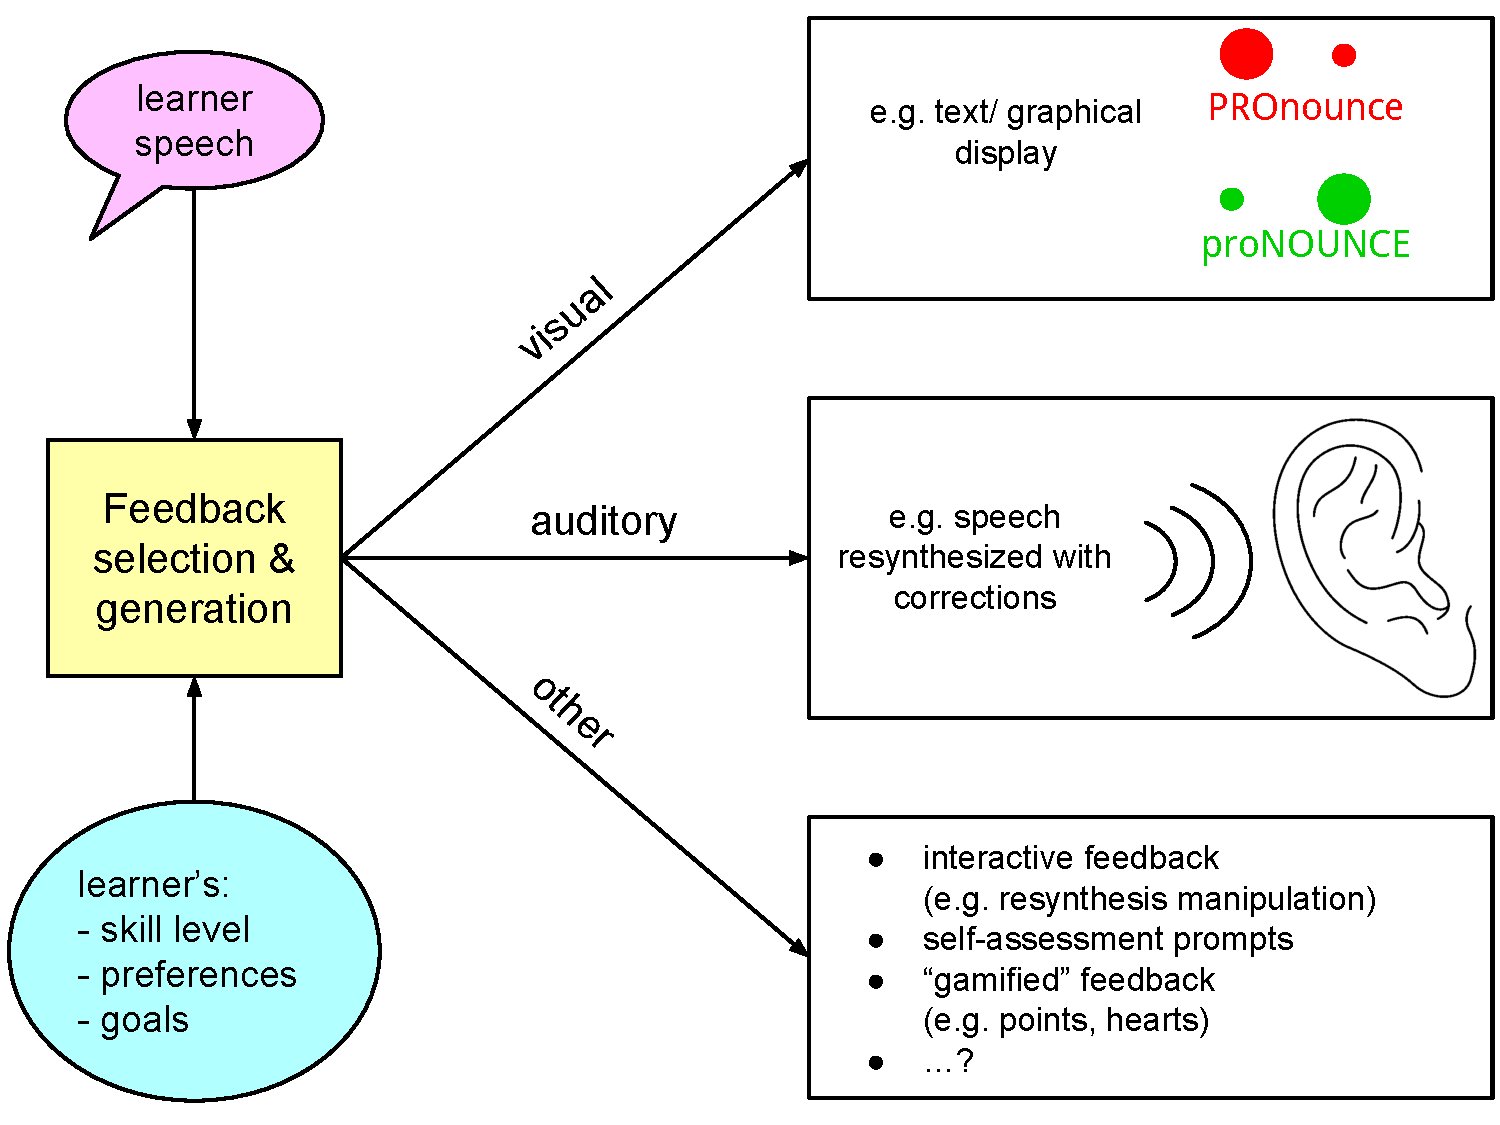
\includegraphics[width=\textwidth]{../img/feedback}
%		\caption{Delivery of prosody feedback in different modalities.}
%		\label{fig:feedback}
%	\end{figure}

%\section{Related work}
%\label{sec:fb:related}
%
%	\cite{Sitaram2011}
%	\cite{Bonneau2011}
%	 	\citep{Hattie2007}


\section{Visual feedback}
\label{sec:fb:visual}

\citep{Sitaram2011}

%TODO replace
%	\subsection{Stylized text}
%	\label{sec:visual:text}
%	
%TODO replace
%	\subsection{Graphical representations of prosody}
%	\label{sec:visual:graphics}
%	
%TODO replace
%	\subsection{Visualizations of the speech signal}
%	\label{sec:visual:visualizations}
	
	As \textcite{Neri2002} point out, waveforms and spectrograms are signal representations designed for speech researchers, not language learners, and the latter may have difficulty understanding these visualizations without the proper training.
	
	Visualizations of the required articulators, such as those displayed in the Fluency pronunciation trainer \citep{Eskenazi2000}, may be helpful for correcting certain segmental errors, but are not likely of much use for correcting lexical stress. 
	
	
\section{Auditory feedback}
\label{sec:fb:auditory}

\citep{Bonneau2011}

\citep{Jilka1998}?

%TODO replace
%	\subsection{Enhanced reference utterance}
%	\label{sec:auditory:enhanced}
%	
%TODO replace
%	\subsection{Resynthesized learner speech}
%	\label{sec:auditory:resynth}
	
	
	
\section{Alternative feedback types}
\label{sec:fb:alternative}

%TODO replace
%	\subsection{Metalinguistic feedback}
%	\label{sec:alternative:metaling}
%	
%TODO replace
%	\subsection{Interactive feedback}
%	\label{sec:alternative:interactive}
%	
%TODO replace
%	\subsection{Implicit feedback}
%	\label{sec:alternative:implicit}


%TODO replace
%\section{Summary}
%\label{sec:fb:summary}